\section{Direct sparse methods}
\label{subseq:sparse methods}

Direct sparse methods combine main advantages of direct and iterative methods i.e. numerical robustness and usage of sparsity structures. As a results, there is no need for preconditioning and the computation complexity is $O(n^2)$ \cite{complexity-of-spdm}. The problem is that storage cost can significantly increase during factorization i.e. the inverse of a sparse matrix can be sufficiently dense. To reduce storage space of $LU$ decomposition this group of methods performs fill-in reduction reodering as a pre-processing step before actual factorization. If storage space is still huge even after fill-in reduction reodering out-of core factorization can be used where partial results are stored in the secondary memory. \\

The most widely known sparse direct method is multifrontal method introduced by \citeauthor{mult-frontal-original:1} in their work \cite{mult-frontal-original:1}. Multifrontal method is an improved extension of a frontal method \cite{frontal-original} that can compute independent fronts in parallel. A front, or also called frontal matrix, can be considered as small dense matrix which is a result of Gaussian Elimination for a particular column. The algorithm, in fact, is as a variant of Gaussian Elimination process. There also exist left-looking and right-looking sparse direct methods. The difference between all of them is explained and can be found in \cite{elimination-tree}.\\


In order to understand and analyze strong scaling behavior of the algorithm we have to briefly discuss the theory of the multifrontal method. For simplicity we will assume that matrix $A$ is real symmetric and $LU$ decomposition boils down to the Cholesky factorization \ref{eq:chol-1}. It allows us to focus on the Cholesky factor $L$ and its sparsity pattern only.

\begin{equation} \label{eq:chol-1}
	A = LDL^T
\end{equation}

The algorithm usually starts with symbolic factorization to predict sparsity pattern of both $A$ and $L$. Once it is done a corresponding elimination tree has to be constructed.\\

\figpointer{\ref{fig:sparsity-pattern-example-mm}}

\begin{figure}[htpb]
  \centering
  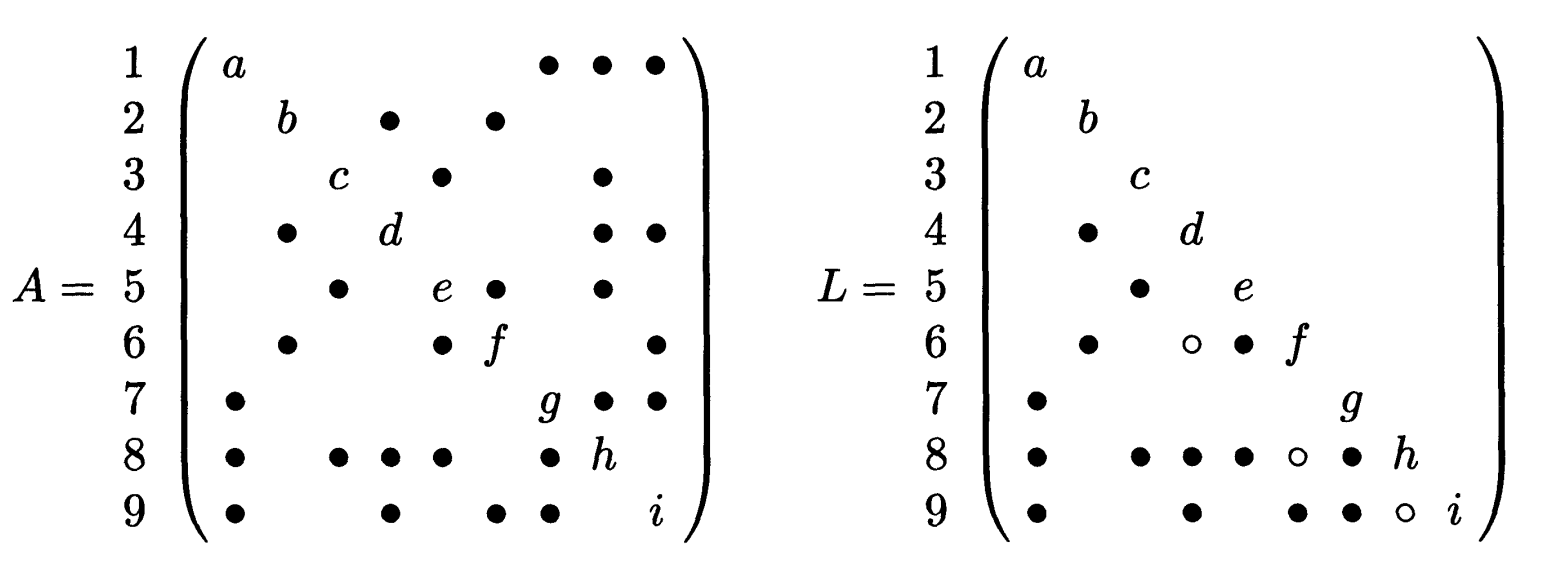
\includegraphics[width=0.9\textwidth]{figures/chapter-2/sparsity-pattern-example-mm.png}
\caption{An example of a sparse matrix and its Cholesky factor \cite{mult-frontal-original:2}}
\label{fig:sparsity-pattern-example-mm}
\end{figure}


Figure \ref{fig:sparsity-pattern-example-mm} shows an illustrative example of a sparse matrix and its Cholesky factor from \cite{mult-frontal-original:2}. The solid circles represent original non-zero elements whereas hollow ones define fill-in factors of $L$. \\


The elimination tree is a crucial part of the method. It can be considered as a structure of $n$ nodes that node $p$ is the parent of $j$ if and only if it satisfies equation \ref{eq:elimination-tree-1}. It is worth pointing out the definition \ref{eq:elimination-tree-1} is not only one possible and one can define a strucutre of an elimination tree in a different way as well. As an example one can find a definition of a general assembly tree in \cite{mult-frontal-original:2} proposed by \citeauthor{mult-frontal-original:2}.\\

\begin{equation} \label{eq:elimination-tree-1}
	p = min(i > j | l_{ij} \neq 0)
\end{equation}


It is important to notice that node $p$ represents elimination process of the corresponding column $p$ of matrix $A$ as well as all dependencies of column $p$ factorization on the results of its descendants.\\


Given definition \ref{eq:elimination-tree-1} we can build the corresponding elimination tree as it is shown in figure \ref{fig:elimination-tree-mm}.\\


\figpointer{\ref{fig:elimination-tree-mm}}

\begin{figure}[htpb]
  \centering
  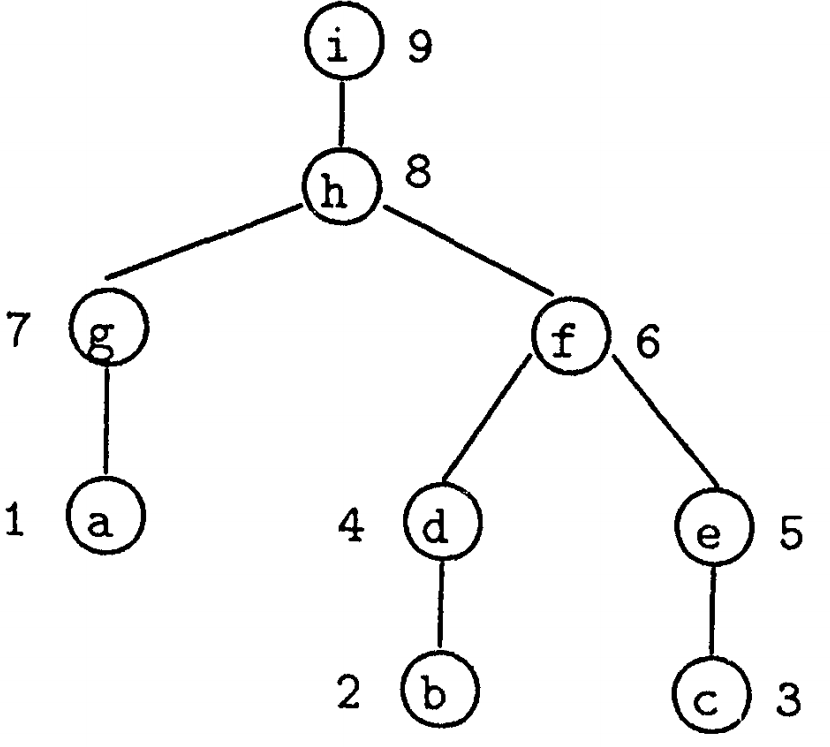
\includegraphics[width=0.45\textwidth]{figures/chapter-2/elimination-tree-mm.png}
\caption{The elimination tree for the matrix example in Figure \ref{fig:sparsity-pattern-example-mm}
 \cite{mult-frontal-original:2}}
\label{fig:elimination-tree-mm}
\end{figure}


The fundamental idea of multifrontal method spins around frontal and update matrices. A frontal matrix is used to perform Gaussian Elimination for a specific column $j$. It is a sum of a frame and update matrices as it can be seen from equation \ref{eq:mm-1}\\.

\begin{equation} \label{eq:mm-1}
	F_{j} = Fr_{j} + \hat{U_{j}} = \begin{bmatrix}a_{j,j} & a_{j,i_1} & a_{j,i_2} & \dots & a_{j,i_r} \\
a_{i_1,j} \\
a_{i_1,j} \\
\vdots & & & 0\\
a_{i_r,j} \\
\end{bmatrix} + \hat{U_{j}}
\end{equation}

where $i_{0}$, $i_{1}$, \dots , $i_{r}$ are the row subscripts of non-zeros in $L_{*j}$ with $i_{0} = j$ and $r$ is number of off-diagonal non-zero elements.\\

The frame matrix $Fr_{j}$ is filed with zeros except the first row and column. The first row and column contain non-zeros elements of the $j$th row and column of the original matrix $A$. Because we consider matrix $A$ to be symmetric the frame matrix is square and symmetric as well.\\

In order to describe parts of the elimination tree we will use the notation $T[j]$ to represent all descendants of the node $j$ in the tree and node $j$ itself. In this way we can define the update matrix $\hat{U_{j}}$ as following:\\

\begin{equation} \label{eq:mm-2}
	\hat{U_{j}} = - \sum_{k \in T[j] -{j}}  \begin{bmatrix}
l_{j,k} \\
l_{i_1,k} \\
\vdots \\
l_{i_1,k} \\
\end{bmatrix} \begin{bmatrix}
l_{j,k} & l_{i_1,k} & \dots & l_{i_1,k}
\end{bmatrix} 
\end{equation}


The update matrix $\hat{U_{j}}$ is, in fact, can be considered as the second term of the Schur complement i.e. update contributions from already factorized columns of $A$.\\

The subscript $k$ represents descendant columns of node $j$. Thus we include and consider only those elements of descendant columns which correspond to the non-zero pattern of the $j$th column that we are currently factorizing.\\

Let's consider the partial factorization of 2-by-2 block dense matrix to better understand essence of update matrix $\hat{U_{j}}$.\\


\begin{equation} \label{eq:mm-3}
A = \begin{bmatrix}
B & V^{T} \\
V & C
\end{bmatrix} 
= 
\begin{bmatrix}
L_{B} & 0 \\
VL^{-T}_{B} & I
\end{bmatrix}
\begin{bmatrix}
I & 0 \\
0 & C - VB^{-1}V^{T}
\end{bmatrix} 
\begin{bmatrix}
L^{T}_{B} & L^{-1}_{B}V^{T} \\
0 & I
\end{bmatrix} 
\end{equation}

Again we assume that $B$ has already been factorized and can be expressed as:

\begin{equation} \label{eq:mm-4}
	B = L_{B}L^{T}_{B}
\end{equation}

The Schur complement from equation \ref{eq:mm-3} can be viewed as the original sub-matrix $C$ and update $-VB^{-1}V^{T}$. It can be written in a vector form as well:

\begin{equation} \label{eq:mm-5}
	-VB^{-1}V^{T} = -(VL^{-T}_{B})(L^{-1}_{B}V^{T}) = - \sum_{k=1}^{j-1}  \begin{bmatrix}
l_{j,k} \\
\vdots \\
l_{n,k} \\
\end{bmatrix} \begin{bmatrix}
l_{j,k} & \dots & l_{n,k}
\end{bmatrix} 
\end{equation}

As it can be easily seen that equations \ref{eq:mm-5} and \ref{eq:mm-2} are identical. The difference is that equation \ref{eq:mm-2} exploits sparsity of the corresponding row and column of $L$ and thus masks unnecessary information. \\

% both eqautions show that the update matrix aggregate all previous information done and in case of the ,ultifrontal methods it means that we aggregate all information from descendants

% Therefore, we can express Uy as an aggregate of outer- product updates from columns in T[Cl],..., T[cs]. 

We can also notice from equation \ref{eq:mm-3} that the frame matrix $Fr_{j}$ corresponds to the block matrix $C$ and brings information from the original matrix $A$ whereas matrix $\hat{U_{j}}$ adds information about the columns that have already been factorized.\\

As soon as the frontal matrix $F_{j}$ is assembled i.e. we have complete update of column $j$, we can perform elimination of the first column and get non-zero entries of factor column $L_{*j}$.\\

Let's denote $\hat{F_{j}}$ as a result of the first column factorization of the frontal matrix $F_{j}$. Then we can express the results as following:\\


\begin{equation} \label{eq:mm-6}
\hat{F_{j}} = \begin{bmatrix}
l_{j,j} & \dots & 0 \\
\vdots & I \\
l_{i_{r},j} \\
\end{bmatrix} 
\begin{bmatrix}
1 & \dots & 0 \\
\vdots & U_{j} \\
0 \\
\end{bmatrix} 
\begin{bmatrix}
l_{j,j} & \dots & l_{i_{r},j} \\
\vdots & I \\
0 \\
\end{bmatrix} 
\end{equation}

where sub-matrix $U_{j}$ represents the full update from all descendants of node $j$ and node $j$ itself. Equation \ref{eq:mm-7} express the sub-matrix $U_{j}$ in a vector form.\\

\begin{equation} \label{eq:mm-7}
\hat{U_{j}} = - \sum_{k \in T[j]}  \begin{bmatrix}
l_{i_1,k} \\
\vdots \\
l_{i_1,k} \\
\end{bmatrix} \begin{bmatrix}
l_{i_1,k} & \dots & l_{i_1,k}
\end{bmatrix}
\end{equation}

Together with the frontal $F_{j}$ and update $\hat{U_j}$ matrices, the update column matrix $U_{j}$ (also called contribution matrices) forms the key concepts of the multifrontal method. To consider the importance of sub-matrix $U_{j}$ let's consider and example illustrated in Figure \ref{fig:information-float}.\\

\figpointer{\ref{fig:information-float}}
\begin{figure}[htpb]
  \centering
  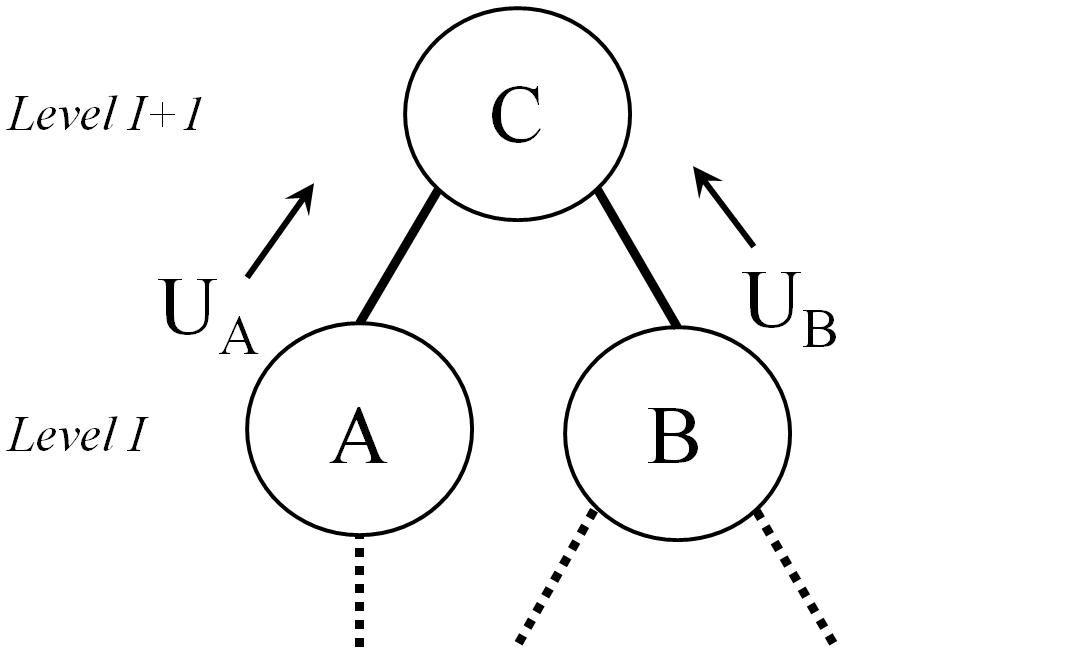
\includegraphics[width=0.45\textwidth]{figures/chapter-2/information-flow.png}
\caption{Information flow of the multifrontal method}
\label{fig:information-float}
\end{figure}


We assume that factorization of columns A and B have already been done and corresponding contribution matrices $U_{A}$ and $U_{B}$ have been computed. From equation \ref{eq:mm-7} we have already known that both $U_{A}$ and $U_{B}$ contain the full updates of all their descendants including updates from factorization of columns $A$ and $B$ as well. Therefore update column matrices $U_{A}$ and $U_{B}$ have already got all necessary information to construct update matrix $\hat{U_{C}}$. The detailed proof and careful explanation can be found in \cite{mult-frontal-original:2}.\\


It might happen that we do not need all rows and columns of $U_{A}$ and $U_{B}$ i.e. we need only some subset of them, because of sparsity of column $C$ . It is also important to place all necessary rows and columns of matrices $U_{A}$ and $U_{B}$ in a right place within matrix $\hat{U_{C}}$. For that reason, an additional matrix operation, called \textbf{\textit{extend-add}}, must be introduced.\\

Let's consider an example from \cite{mult-frontal-original:2} of an extend-add operation for 2-by-2 matrices $R$ and $S$ which correspond to the indices ${5,8}$ and ${5,9}$ of some matrix $B$, respectively.\\

\begin{equation}
R = \begin{bmatrix}
p & q \\
u & v \\
\end{bmatrix} 
,
\:
S = \begin{bmatrix}
w & x \\
y & z \\
\end{bmatrix} 
\end{equation}

The result of the operation is going to be a 3-by-3 $K$ matrix which looks as following:\\

\begin{equation} \label{eq:mm-8}
K = R \extendadd S = \begin{bmatrix}
p & q & 0 \\
u & v & 0 \\
0 & 0 & 0 \\
\end{bmatrix} 
+
\begin{bmatrix}
w & 0 & x \\
0 & 0 & 0 \\
y & 0 & z \\
\end{bmatrix} 
=
\begin{bmatrix}
p + w & q & x \\
u & v & 0 \\
y & 0 & z \\
\end{bmatrix} 
\end{equation}

Hence we can express formation of the frontal matrix $F_{j}$ using the extend-add operation and all direct children of node $j$ in the following way:


\begin{equation} \label{eq:mm-9}
	F_{j} = \begin{bmatrix}a_{j,j} & a_{j,i_1} & a_{j,i_2} & \dots & a_{j,i_r} \\
a_{i_1,j} \\
a_{i_1,j} \\
\vdots & & & 0\\
a_{i_r,j} \\
\end{bmatrix} \extendadd U_{c_1} \extendadd \dots \extendadd U_{c_s} 
\end{equation}

where $c_{1}, \: c_{2}, \: \dots \: c_{n}$ are indices of direct children of the node $j$.\\

Now it can be clearly seen that the resultant frontal matrix $F_{j}$ is a small dense one and it can be efficiently computed using BLAS level 3 subroutines.\\

After factorization we have to build the contribution matrix $U_{j}$ i.e. add columns and rows of $U_{c_1}, \:, U_{c_2}, \: \dots, U_{c_s}$ to $U_{j}$ that have not been used in factorization of $F_{j}$ due to sparsity of column $j$. After that we can continue to move up along the tree. 
The complete update matrices grow in size as we move to the top of the tree. Therefore they have to be stored in a sparse matrix format to stay within memory constrains of the computer.\\


Another important aspect is storage and manipulation of frontal and contribution matrices. Sometimes we have to store contribution matrices produced in previous steps into some temporary buffer and efficiently retrieve them later during factorization. This can require some matrix re-ordering. In case of symmetric matrices, one can apply postordering on a tree to be able to use the stack data structure to alleviate the process of contribution matrix manipulations during factorization. A tree postordering is based on topological ordering and it has been proven that it is equivalent to the original matrix ordering and thus leads to the same filled graph \cite{mult-frontal-original:2}. \todo{sentence refactoring} We refer to the original matrix ordering as the ordering received from fill-in reduction operation.\\


A tree postordering means that a node is ordered before its parent and, additionally, nodes in each subtree are numbered consecutively. Figure \ref{fig:mm-matrix-postordering} shows an example of posrordering applied to the elimination tree of the matrix from figure \ref{fig:sparsity-pattern-example-mm}. The results of this can be see in figure \ref{fig:mm-contrib-matrix-manipulation} where consecutive \textit{push} and \textit{pop} operations are efficiently used during factorization and thus simplify the program logic.\\


\figpointer{\ref{fig:mm-matrix-postordering}}
\begin{figure}[htpb]
  \centering
  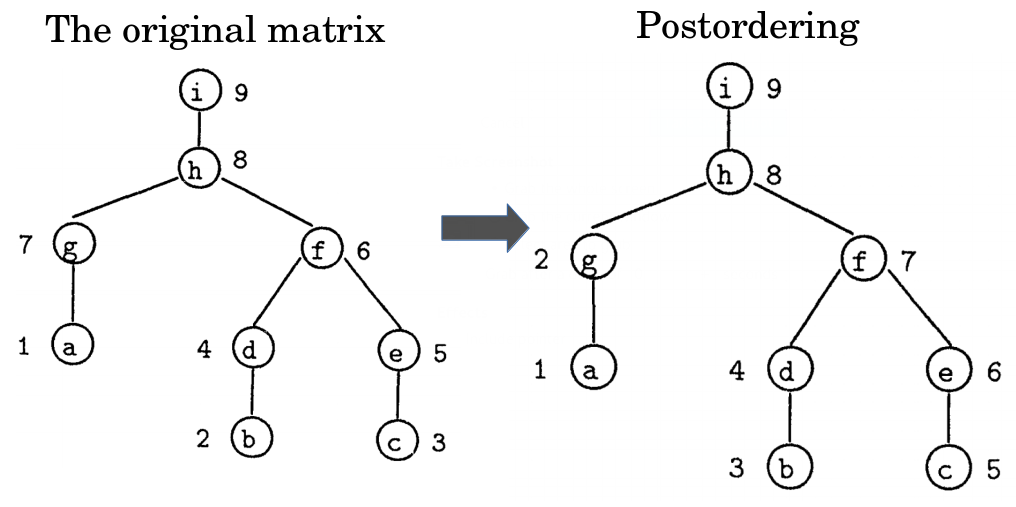
\includegraphics[width=0.75\textwidth]{figures/chapter-2/elimination-tree-mm-postordering.png}
\caption{An example of matrix postordering from \cite{mult-frontal-original:2}}
\label{fig:mm-matrix-postordering}
\end{figure}


\figpointer{\ref{fig:mm-contrib-matrix-manipulation}}
\begin{figure}[htpb]
  \centering
  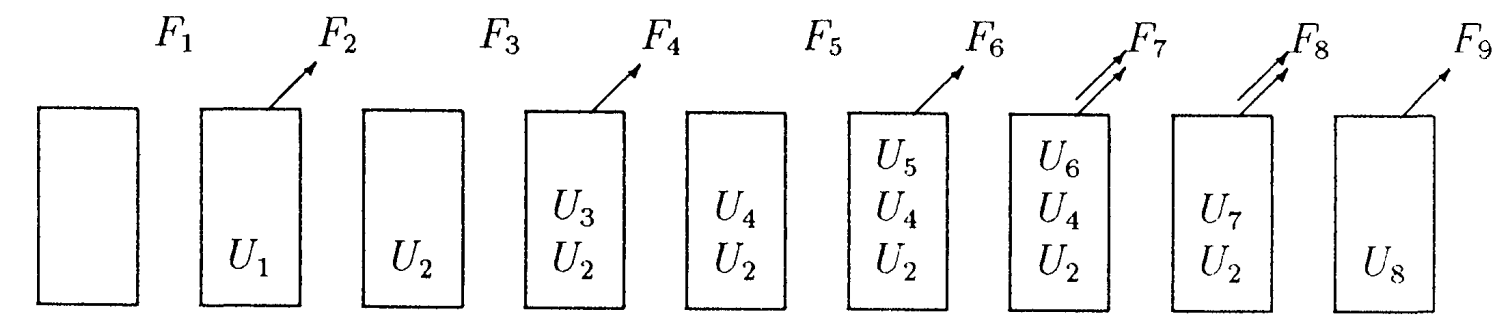
\includegraphics[width=0.75\textwidth]{figures/chapter-2/mm-contrib-matrix-manipulation.png}
\caption{The stack contents for the postordering \cite{mult-frontal-original:2}}
\label{fig:mm-contrib-matrix-manipulation}
\end{figure}


We can see the algorithm requires to perform some preprocessing steps in order to estimate the size of working space for matrix manipulations. If the working space has not been predicted correctly the algorithm will terminate during factorization. Additionally it can happen that even with the correct estimation we can be run out of space in the main memory, in case of huge sparse matrices. This fact can require to use the secondary memory and, as a result, the execution time will increase significantly. Therefore, different optimal postordering schemes have been proposed which allow to shrink the amount of space needed during factorization \cite{mm:optimal-tree-postordering} \cite{mm:elimination-tree-rotations}. Some schemes, for example elimination tree rotations \cite{mm:elimination-tree-rotations}, can lead to deep and unbalanced trees which might have their negative effect on task parallelism as we will see later.\\


In general, the estimation of working space can be tricky due to pivoting. Because pivoting happens only during the numerical factorization phase it is not always possible to estimate enough space correctly during the analysis one. There exist some heuristics which allow to use some numerical matrix information during symbolic factorization to better predict the amount of required space \cite{wsmp:direct-solution-of-general-system}.\\


% supernodal
In practice, an improved version of multifrontal method, called supernodal method, is used. The idea of the supernodal method is to shrink the final elimination tree by grouping some particular nodes/columns in one computational unit. As a result, more useful floating point operations per memory access can be performed by eliminating few columns at once within the same frontal matrix.\\

A supernode is formed by a set of contiguous columns with identical off-diagonal sparsity structure forms. Thus, a supernode has few important properties. Firstly, it can be expressed as a set of indices, namely: $\{j, \: j+1, \: \dots, \:j + t\}$, where node $j + k$ is	parent of $j + k - 1$ in the elimination tree. Secondly, the size of the supernodal frontal matrix is equal to the frontal matrix of the $j$th column within a supernode. As an example, Figure \ref{fig:supernodal-method-postordering-and-etree} shows a postordered matrix $A$ and its Cholesky factor $L$ as well as the corresponding supernodal elimination tree.


\figpointer{\ref{fig:supernodal-method-postordering-and-etree}}

\begin{figure}[htpb]
  \centering
  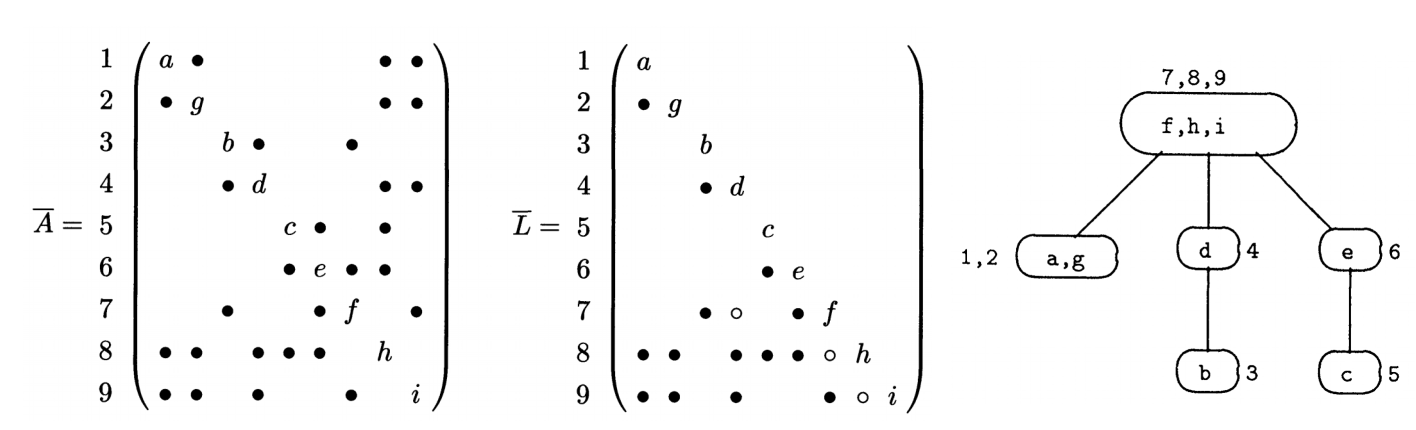
\includegraphics[width=1.0\textwidth]{figures/chapter-2/supernodal-method-postordering-and-etree.png}
\caption{An example of a supernodal elimination tree \cite{mult-frontal-original:2}}
\label{fig:supernodal-method-postordering-and-etree}
\end{figure}
 
 
Equation \ref{eq:mm-10} expresses the building process of a frontal matrix of a supernode. In contrast to \ref{eq:mm-9}, the frame matrix $\mathcal{F}_{j}$ contains more dense rows and columns. As before, we use \textit{extend-add} operation to get the full block update from children contribution matrices.\\


\todo{check grammar}
It should be mentioned there exist more sophisticated variants of supernodes. Most of the time, it intends to improve efficiency of the algorithm. \citeauthor{mult-frontal-original:2} pointed out that supernodes could be defined without using the contiguous constrains \cite{mult-frontal-original:2}. On another hand, \citeauthor{complexity-of-spdm} defines supernodes corresponded to separators from the nested dissection step  \cite{complexity-of-spdm} which was used for fill-in reduction.\\



 \begin{equation} \label{eq:mm-10}
	\mathcal{F}_{j} = \begin{bmatrix}a_{j,j} & a_{j,j+1} & \dots & a_{j,j+t}  & a_{j,i_1} & \dots & a_{j,i_r} \\
a_{j+1,j} & a_{j+1,j+1} & \dots & a_{j+1,j+t}  & a_{j+1,i_1} & \dots & a_{j+1,i_r} \\
\vdots & \vdots & \dots & \vdots \\
a_{j+t,j}  & a_{j+t,j+1} & \dots & a_{j+t,j+t}  & a_{j+t,i_1} & \dots & a_{j+t,i_r} \\
a_{i_1,j} & a_{i_1,j+1} & \dots & a_{i_1,j+t} \\
\vdots & \vdots & \dots & \vdots  & & 0\\ 
a_{i_r,j} & a_{i_r,j+1} & \dots & a_{i_r,j+t} \\
\end{bmatrix} \extendadd U_{c_1} \extendadd \dots \extendadd U_{c_s} 
\end{equation}


Up to this point we have already seen all key concepts of the multifrontal method and discussed how the algorithm works. We will move to the discussion of parallelization of the method. \\


The elimination tree, in fact, represents dependencies among columns. Conversely, the tree also shows independent steps of elimination process. Hence the tree forms independent problems that can be executed in parallel. Task parallelism is the main and primary source the algorithm parallelisation. Figure \ref{fig:elimination-tree-mm-parallel-steps} shows task parallelism, for the example given in Figure \ref{fig:supernodal-method-postordering-and-etree}, where each color represents a set concurrent tasks.\\


\figpointer{\ref{fig:elimination-tree-mm-parallel-steps}}

\begin{figure}[htpb]
  \centering
  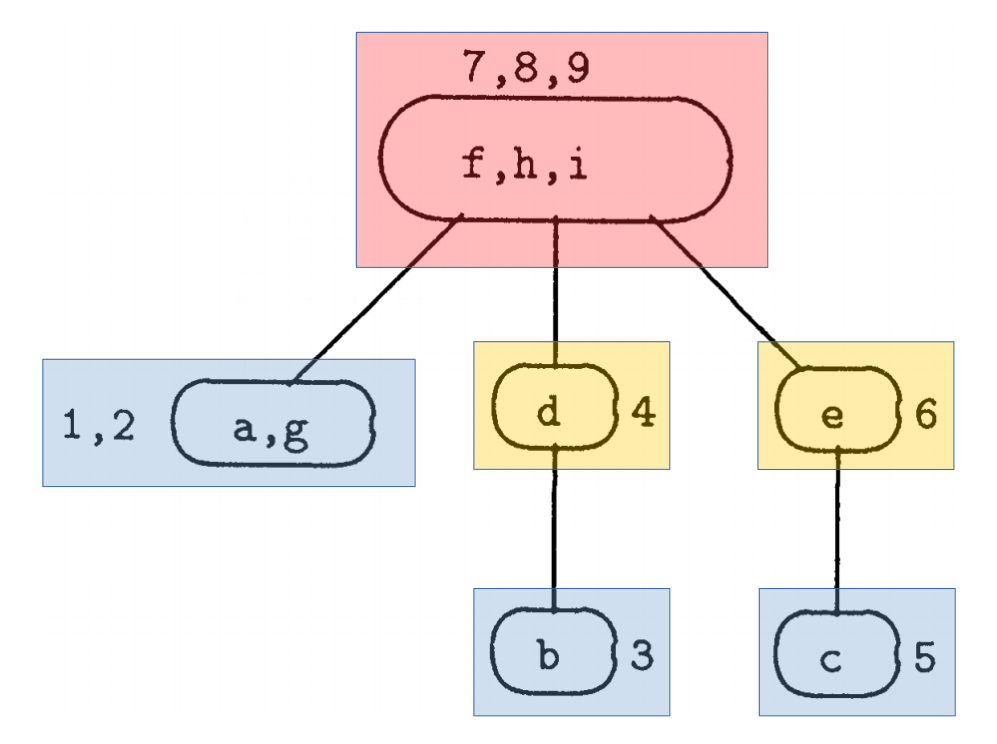
\includegraphics[width=0.5\textwidth]{figures/chapter-2/elimination-tree-parallel.png}
\caption{Parallel steps of the multifrontal method based on the example in Figures \ref{fig:supernodal-method-postordering-and-etree}}
\label{fig:elimination-tree-mm-parallel-steps}
\end{figure}


For example, nodes on separate branches of the tree are totally independent and can processed in parallel. However, as soon as at least two branches run into the same node it forms a dependency and we have to wait all contribution matrices of its children and cannot proceed further.\\ 


We can observe the amount of task parallelism is rapidly decreasing while moving towards the root along the tree. Once we reach the root of the tree the algorithm becomes totally sequential. This fact can play the significant role in strong scaling behavior of the method.\\


We developed two simple models based on perfectly balanced binary trees to better understand strong scaling of the algorithm. The main concept of the models is so-called cost per level or cost per node. This idea is similar to the recursion trees in \cite{recursion-tree} which explains and computes complexity of recurrent algorithms.\\


Figure \ref{fig:mm-parallel-model-tree-linear} represents the first model where we keep the same cost per level whereas the second model (Figure \ref{fig:mm-parallel-model-tree-quadratic}) simulates quadratic cost decay from level to level. Additionally we assume that computational cost distributed uniformly between nodes at the same level for both models.\\


\figpointer{\ref{fig:mm-parallel-model-tree}}
\begin{figure}
\centering
	\begin{tabular}{cc}
			\subfloat[Model 1: equal cost per level]{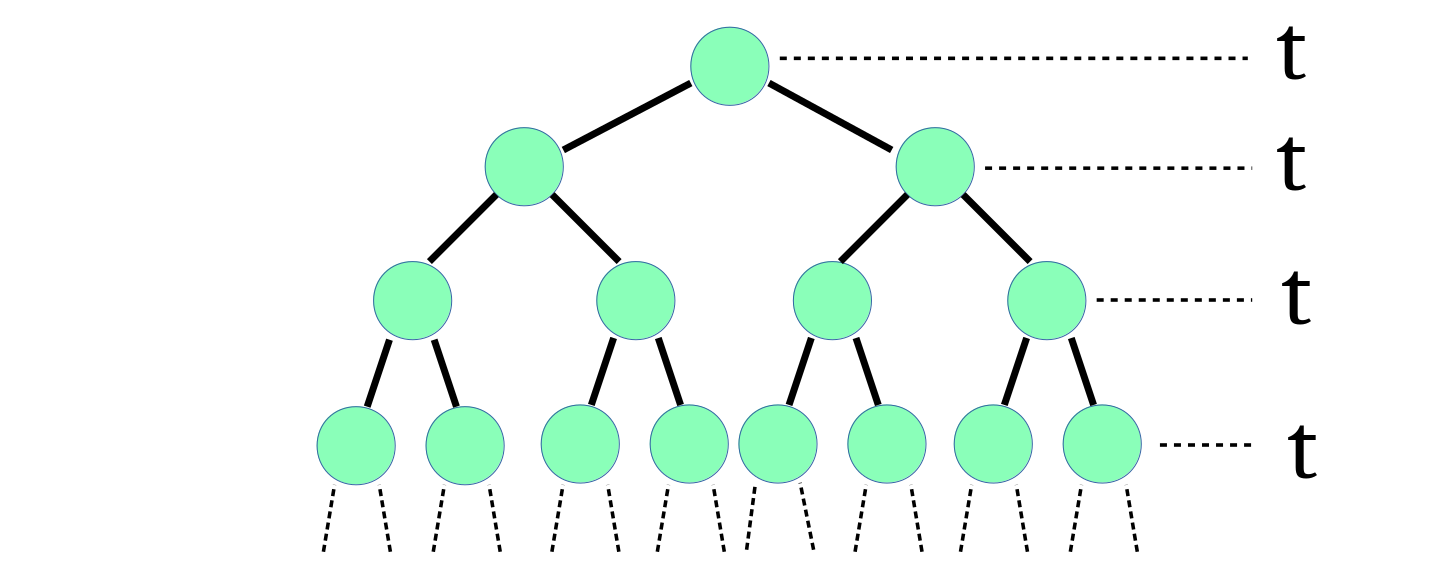
\includegraphics[width=0.5\textwidth]{figures/chapter-2/mm-parallel-model-tree-1.png} \label{fig:mm-parallel-model-tree-linear}} & 
		\subfloat[Model 2: quadratically decreasing cost per level]{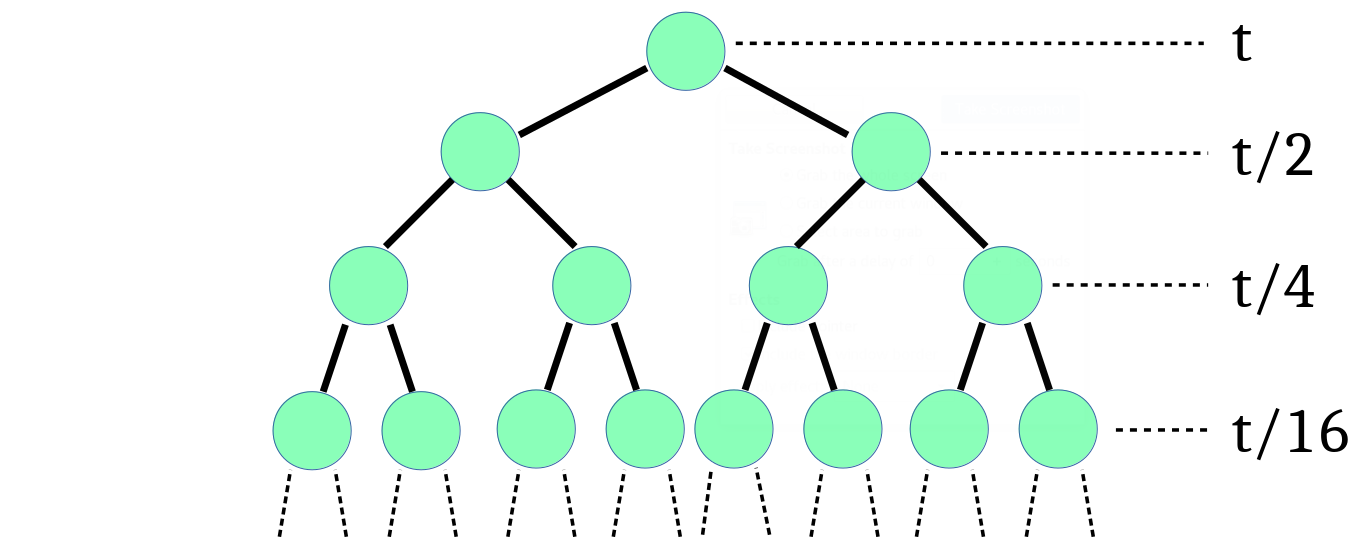
\includegraphics[width=0.5\textwidth]{figures/chapter-2/mm-parallel-model-tree-2.png} \label{fig:mm-parallel-model-tree-quadratic}} \\
	\end{tabular}
	\caption{Simple parallel models of the multifrontal method}
	\label{fig:mm-parallel-model-tree}
\end{figure}

\todo{sentence refactoring}
We have to say that our models mimic only numerical factorization and do not include time spent on any per-processing steps, for example, fill-in reduction reodering. A cost per level can be interpreted in different ways e.g. increase of partial factorization time due to growth of frontal matrices in size, time increase spent on numerical pivoting, increase of MPI communication overheads due to growth of contribution matrices, etc. It should be mentioned that real computer implementations of the multifrontal algorithm (MUMPS, SuperLU, etc.) are quite sophisticated in many aspects and our models do not have any intention to analyze performance of a particular package. Instead the objective of these models is to show possible strong scaling behavior and possible bottlenecks. \\


We will consider only task parallelism at the beginning to a first approximation and later we will discuss how additional data parallelism can affect algorithm performance.\\

% assumtion that cost is equal within the level!!!

Instead of coloring given in Figure \ref{fig:elimination-tree-mm-parallel-steps}, we assume that each level has the same color and thus can be executed fully in parallel if we have enough processing elements. We cannot go to the next level till the current one has not been completed yet i.e. free processing elements, that do not have nodes to execute at the current level, have to wait.\\


As we mentioned above the root of the tree can be processed purely sequentially if we only consider task parallelism. As a first approximation, time spent on the root factorization determines the minimal execution time according to the Amdahl's low \cite{wiki:amdahls-low}. More precisely, the minimal execution time is equal to a sum of time spent on single node partial factorization at each level. This time determines the asymptote on the corresponding speed-up graph.\\


We considered a perfectly balanced tree with 16 levels, 65535 nodes and the maximum of 20 processing elements as an example. The numerical results of linear and quadratic models can be viewed in Figures \ref{fig:mm-parallel-model-tree-linear} and \ref{fig:mm-parallel-model-tree-quadratic}, respectively. The figures show a rapid drop of performance, especially in case of the quadratic model. Table \ref{table:mm-potential-model-speed-up} demonstrates the maximum potential speed-up, having 32768 processing elements which is equal to the number of leaves of the tree, against the speed-up we have got using only 20 processing elements.\\


\figpointer{\ref{fig:mm-parallel-model-speed-up}}
\begin{figure}
\centering
	\begin{tabular}{cc}
			\subfloat[Theoretical speed-up of Model 1]{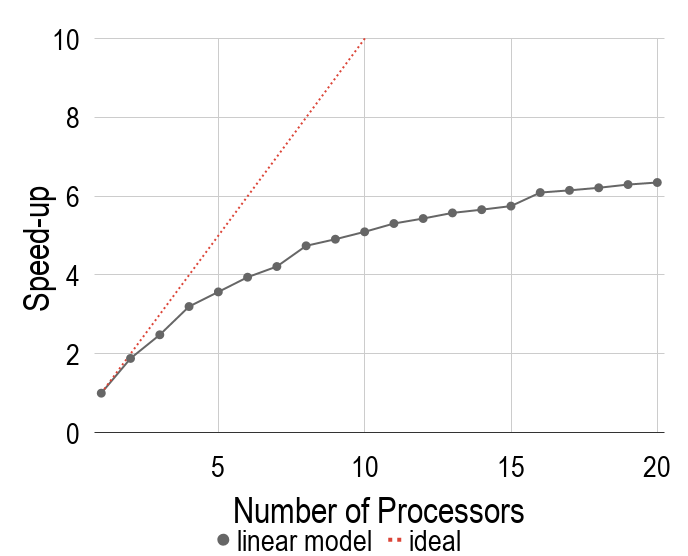
\includegraphics[width=0.45\textwidth]{figures/chapter-2/mm-parallel-model-tree-1-speedup.png}} &
		\subfloat[Theoretical speed-up of Model 2]{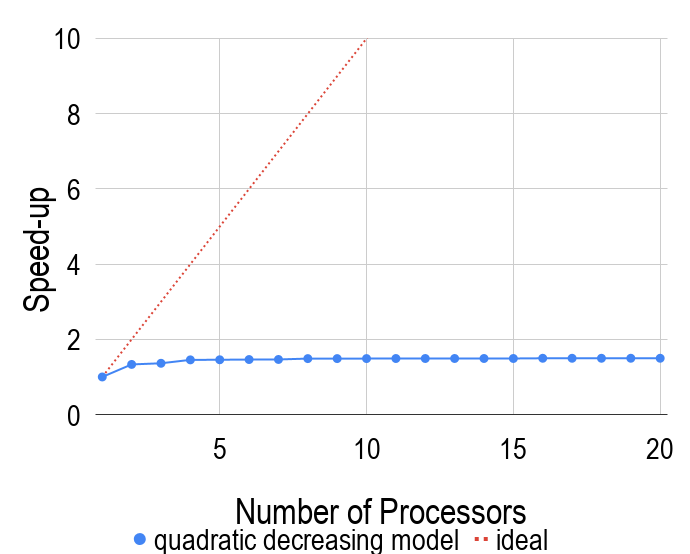
\includegraphics[width=0.45\textwidth]{figures/chapter-2/mm-parallel-model-tree-2-speedup.png}} \\
	\end{tabular}
	\caption{Theoretical speed-up}
	\label{fig:mm-parallel-model-speed-up}
\end{figure}


\begin{table}[htpb]
\centering
\begin{tabular}{|c|c|c|}
\hline
        & 20 PEs  & 32768 PEs \\ \hline
Model 1 & 6.3492  & 8.0000    \\ \hline
Model 2 & 1.4972 & 1.5000   \\ \hline
\end{tabular}
\caption{Potential speed-up of linear and quadratic models}
\label{table:mm-potential-model-speed-up}
\end{table}


We can see that model 1 still has some potential to grow whereas the second model has already reached its asymptote and further increase of processing elements does not make sense. In spite of a potential growth of the first model, both models have very low parallel efficiency even with 20 processing elements which can be observed from table \ref{table:mm-model-efficiency-20-pe}.\\


\begin{table}[htpb]
\centering
\begin{tabular}{|c|c|}
\hline
        & 20 PEs \\ \hline
Model 1 & 0.3175 \\ \hline
Model 2 & 0.0749 \\ \hline
\end{tabular}
\caption{Efficiency of linear and quadratic models using 20 PEs}
\label{table:mm-model-efficiency-20-pe}
\end{table}


Both models shows that computational intensity per node grows from bottom to top. It is easy to conclude from Figure \ref{fig:mm-parallel-model-tree} that intensity per node is equal $t/2^{i}$ and $t/2^{2i}$ for the first and second models, respectively (where $i$ is a level of the tree). It reflects that the most intensive part of the method is centered on the top part of the tree i.e. first few level. \citeauthor{mult-frontal-original:2} discussed application of the multifrontal method to a $k-by-k$ regular model problem with nine-point difference operator in his paper \cite{mult-frontal-original:2}. He observed that factorization of the last 6 nodes took slightly more than 25\% of the total amount of arithmetical operations. As a comparison, table \ref{table:mm-simple-model-work-load} shows fractions of time spent on processing first few top levels of our models: 1 and 2.\\


\begin{table}[htpb]
\centering
\begin{tabular}{|c|c|c|}
\hline
        & Model 1 & Model 2 \\ \hline
Level 0 & 6.25\%  & 50.00\% \\ \hline
Level 1 & 12.50\% & 75.00\% \\ \hline
Level 2 & 18.75\% & 87.50\% \\ \hline

\end{tabular}
\caption{Distribution workload per level in case model 1 and 2}
\label{table:mm-simple-model-work-load}
\end{table}


As we can see, the result of our first model is relatively close to 25\% and, therefore, it looks quite optimistic. However, the second model shows that 87\% of workload is focused on the top part of the tree and, as a result, we can consider that model as extremely pessimistic. \\


By and large, reduction of time spent on the top nodes is a way to improve strong scaling behavior. To do so, data parallelism can be additionally exploited for these nodes. It is worth noting that data parallelism at bottom levels does not make sense because it leads to increase of granularity there and thus increase communication overheads which can lead to significant performance drop.\\


Figure \ref{fig:mumps-task-data-parallelism} shows an example of two types of parallelism applied to the algorithm. First of all, we can see the leaves are grouped in subtrees and a single PE is assigned to each subtree. Other nodes are distributed among three different types. Nodes of the first type uses task parallelism only, which is induced by the tree, and each node is executed in a single processor. The second type exploits data parallelism with 1D block row distribution among the processors. The root belongs to the third type where data parallelism is used with 2D block cyclic distribution. The details of MUMPS parallelism management is carefully explained and can be found in \cite{mumps:task-data-parallelism}.\\


\figpointer{\ref{fig:mumps-task-data-parallelism}}

\begin{figure}[htpb]
  \centering
  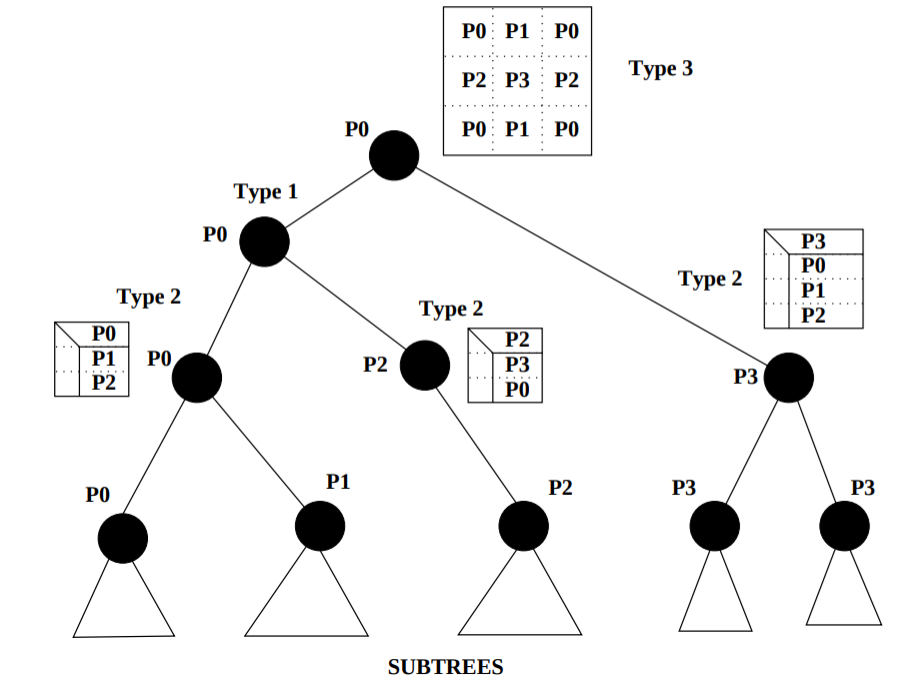
\includegraphics[width=0.65\textwidth]{figures/chapter-2/mumps-task-data-parallelism.png}
\caption{MUMPS parallelism management in case of 4 PEs \cite{mumps:task-data-parallelism}}
\label{fig:mumps-task-data-parallelism}
\end{figure}


All the techniques mentioned above were designed to improve strong scaling behavior by splitting the most intensive parts among all available processors. Going back to our models, we can also think about that in a slightly different way, namely: \textit{data parallelism helps to re-distribute cost per node/level on the corresponding elimination tree}. However, we have to notice that efficiency of data parallelism totally depends on sizes of frontal matrices at the top part of the tree. In case of skinny sparse matrices, oversubscription of processing elements can lead to strong performance penalties as we could see from section \ref{subseq:direct methods}. A machine-dependent minimal frontal matrix size was introduced in MUMPS in order to control whether to use ScaLAPACK at the root node or not \cite{mumps-manual}. It can happen that the algorithm uses only task parallelism, due to the threshold, and, as a results, scaling will only depend on the tree structure that can be deep and unbalanced.\\


Figure \ref{fig:model-1-vs-mumps} shows comparison of strong scaling between model 1 and parallel numerical factorization of the matrix \textit{\textbf{cant}} done with using MUMPS library. The matrix has been downloaded from SuiteSparse Matrix Collection \cite{sparse-matrix-collection:1}, \cite{sparse-matrix-collection:2}. The sparsity pattern before and after fill-in reduction is shown in figure \ref{fig:cant-matrix-sparsity-pattern}. Parameters of the matrix are listed in table \ref{table:matrix-cant-parameters}.


\begin{table}[htpb]
\centering
\begin{tabular}{|c|c|c|c|}

\hline
Matrix Name     & n     & nnz     & nnz / n \\ \hline
cant & 62451 & 4007383 & 64.1684 \\ \hline

\end{tabular}
\caption{Parameters of the matrix \textit{\textbf{cant}}}
\label{table:matrix-cant-parameters}
\end{table}


\figpointer{\ref{fig:model-1-vs-mumps}}
\begin{figure}[htpb]
  \centering
  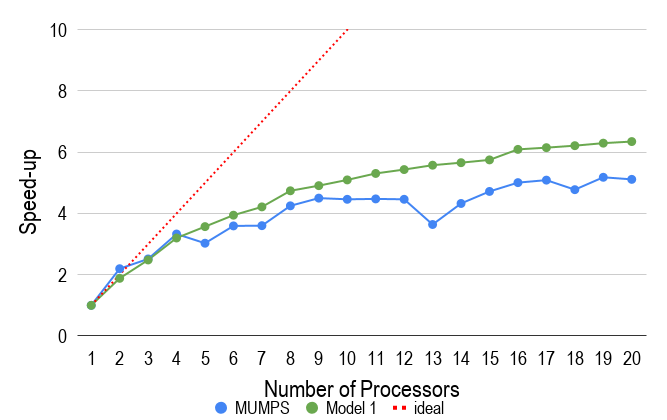
\includegraphics[width=0.65\textwidth]{figures/chapter-2/model-1-vs-mumps.png}
\caption{Comparison between model 1 and numerical factorization of the matrix \textit{\textbf{cant}} using MUMPS library}
\label{fig:model-1-vs-mumps}
\end{figure}


\figpointer{\ref{fig:cant-matrix-sparsity-pattern}}
\begin{figure}[htpb]
  \centering
  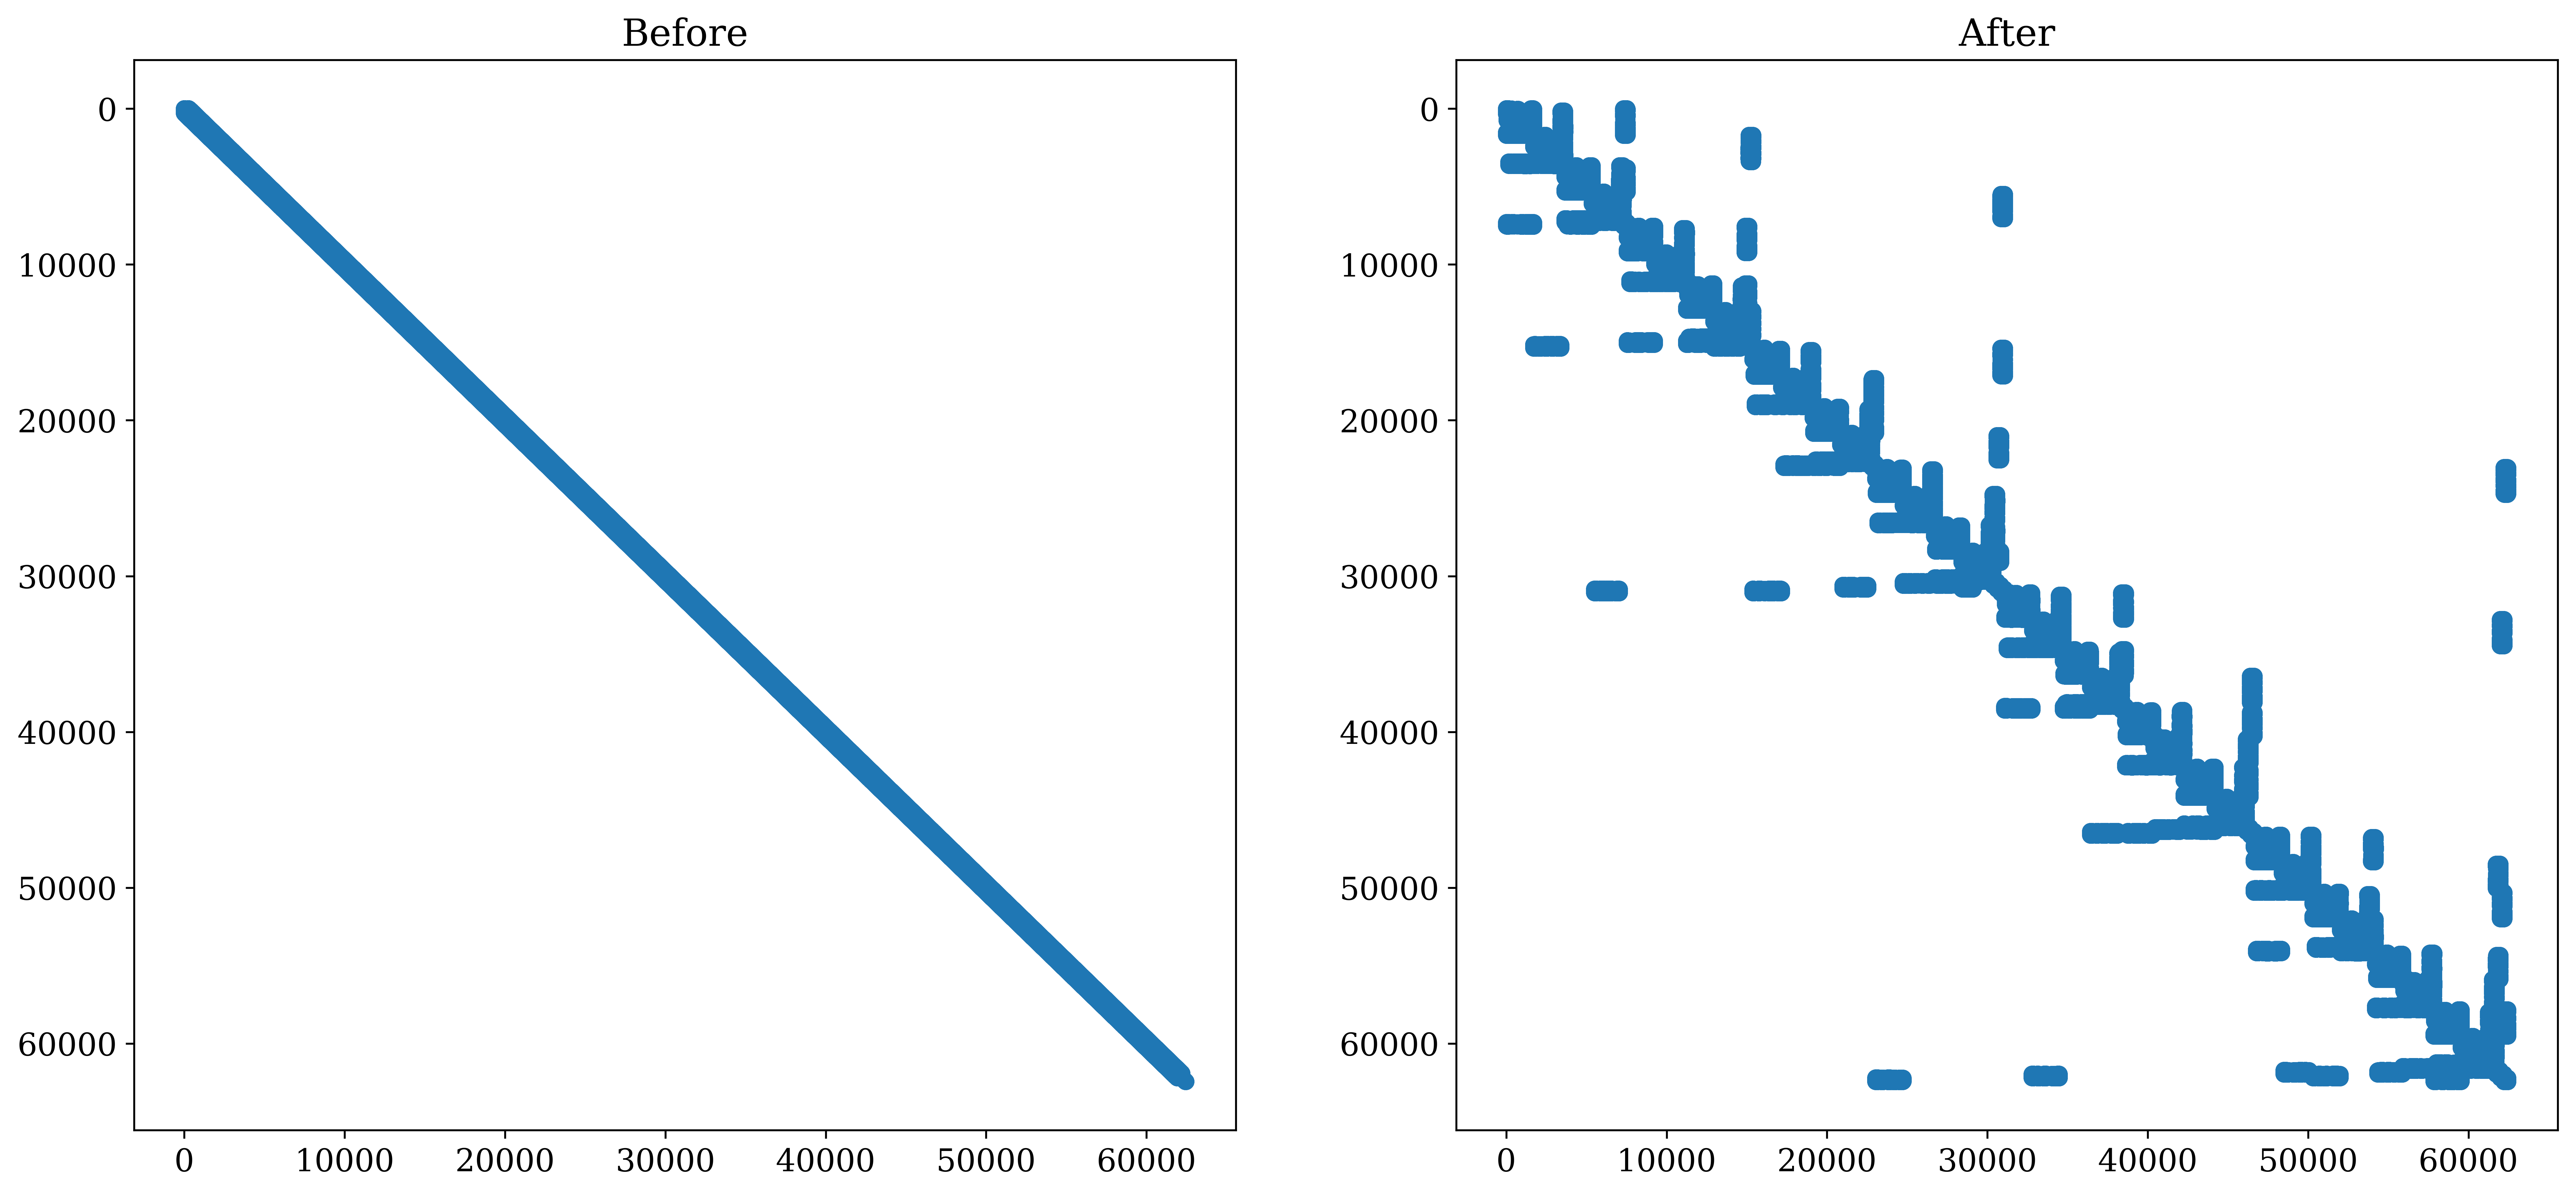
\includegraphics[width=1.00\textwidth]{figures/chapter-2/cant-matrix-sparsity-pattern.png}
\caption{Sparsity structure of the matrix \textit{\textbf{cant}} before and after fill-in reduction}
\label{fig:cant-matrix-sparsity-pattern}
\end{figure}




As we can see, our model and the experiment show the same trend and the results are pretty much close to each other. However, our model takes into consideration only task parallelism whereas MUMPS exploits both data and task parallelism. Additionally, we have to mention that our model 1 works well only for relatively big sparse matrices. It can be quite inaccurate in case of small/skinny sparse systems. \\


In general, it is possible to refine our models and make them more accurate, using Bulk Synchronous Parallel (BSP) approach, for example. However, it will require to possess a real postordered elimination tree, extracted from a specific implementation of multifrontal method, together with information about supernodes sizes. We strongly believe the new enhanced model can explain the jagged strong scaling behavior of the MUMPS solver that we can observe in figure \ref{fig:model-1-vs-mumps}. But, this approach seems to be quite cumbersome and requires to delve into the source code of a particular library. It is needless to say that data can be retrieved only during run time and only after the analysis phase. This makes it less valuable and we can see that it is definitely a wrong way to go.\\


There are few important aspects to discuss at the end of the section. Numerical robustness is the main advantage of the multifrontal method. It does not require any preconditioner to solve a system of equations. As we discussed in the previous section, tuning a specific preconditioning algorithm can take a considerable amount of time, especially in case of our systems. As another advantage, the method (heavily) exploits matrix sparsity which lowers computational complexity up to $O(n^2)$. In case of massively huge matrices, the algorithm can utilize the secondary memory which sometimes is only one way to solve a system.\\


We can conclude, from the analysis above, the method has inherently bad scaling behavior and it is quite sensitive to a matrix structure. We will see later that it is almost impossible to predict the saturation point i.e. a point after which performance either drops or stays at the same level. We assume that scaling becomes better with growth of a matrix size. However, we cannot expect such behavior for small and medium systems.\\  


Secondly, we can see the algorithm requires many pre-processing steps to be done before numerical factorization phase. All these steps must run in parallel and be highly scalable. Apart from performance constrains of the steps, they must lead to wide and well balanced elimination trees which becomes crucial during the numerical phase.\\


Lastly, the algorithm can fail due to incorrect  working space prediction. As a results, factorization has to be restarted with some modification of input solver parameters.\\

























